\chapter{Deep Learning in Digital Histopathology}
Manual analysis of histopathology slides is expensive, takes long time to complete and requires highly trained professionals and quality assurance by performing peer reviews \cite{Wemmert2021}. With the invention of virtual microscopy, which enables H\&E stained glass slides to be converted into digital slides, and the introduction of Whole-slide Images (WSIs), the field is entering a new era. The term Digital Pathology or Digital Histopathology is often being used. In Digital Pathology, much effort is put into developing tools that would help medical experts to semi- or fully automate the visual analysis of the digital slides. Entities such as different tissue types and cells can be identified and classified.

Deep learning has shown extreme potential in many areas, including medicine and processing of medical image data \cite{LeCun2015}.

\section{Architectures}
Neural network architectures like Convolutional Neural Networks \cite{LeCun2015-2} and U-Net \cite{Ronneberger2015} have proven to be effective in medical image analysis \cite{Santosh2022-2}. In recent years, also a concept of Vision Transformers \cite{Dosovitskiy2020, Hu2023} used in medical imaging shows promising results \cite{Shamshad2023, Hu2023, He2023}. In further sections we describe each architecture and its contribution to the analysis of medical images and Digital Pathology.

\subsection{Convolutional Neural Networks}
In 1959, Hubel and Wiesel conducted experiments that inspired the advent of the Convolutional Neural Networks (CNN). In their experiments, they put a microelectrode into a cat's brain (into the part called primary visual cortex), while it was under partial anaesthesia. While showing various images to it, they measured the neurological activity of the cortex \cite{Hubel1959}. According to the results, a hierarchical pattern can be observed in the activity of the visual cortex, where the neurons close to the retina captured the simplest patterns (like different illuminations and lines under various angles) and the farther layers  captured more complex patterns (like geometric shapes and other complex visual patterns) \cite{Hubel1959}. 

CNNs took advantage of these findings and rebuilt the classical neural network layers to be able to capture more complex features with increasing depth. They utilize so-called convolution layers along with the ReLU activation function to learn to extract relevant features from the image. The deeper the convolution layer, the more complicated features it can learn \cite{Santosh2022-2}. 

Similarly to the Hubel and Wiesel cat's visual cortex, the first layers can learn to identify basic shapes like lines and simple geometric shapes, and the deeper layers can learn to identify more complex ones. Such an example of CNN is shown in figure \ref{fig:cnn}.

\begin{figure}[H]
\begin{centering}
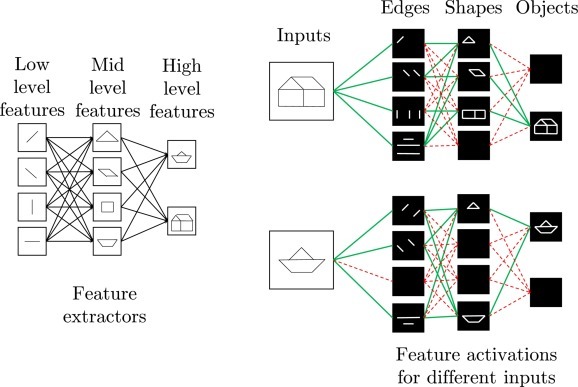
\includegraphics[width=8cm]{assets/images/cnn.jpg}
\par\end{centering}
\caption{Example of CNN learning strategy \cite{Santosh2022-2}}
\label{fig:cnn}
\end{figure}

A convolution layer applies a series of operations on its input and produces an activation map. The most important part is applying a kernel, which is a tensor of fixed width and height, over the input image or activation from the previous convolution layer. This fundamental operation serves as a feature-extracting technique. The kernel slides over its input across its height and width and at each step it performs element-wise multiplication of the pixel values it currently overlaps at each layer of depth and then sums them together to produce a single value. So, for example, if the input is of size $100\times100\times3$ (standard RGB image with 3 channels for red, green, and blue colour), then the kernel is applied to all three channels simultaneously. After the kernel is applied to the whole image, the resulting activation filter will be of size $100\times100\times1$ (assuming that other hyperparameters of convolution are configured in such a manner that original width and height remain unchanged for the activation map - we will cover them later in this chapter), because the kernel will collapse its depth. 

The kernel filters can be handcrafted to multiply and intensify certain properties of the image. Examples include the Prewitt, Gabor, Sobel, Laplacian, and Roberts filters for edge and gradient detection. In standard image processing, the weights inside of the kernel are preset. However, in the CNNs these weights are learned during training, so the network determines what features of the image the activation maps will be focused on and hence the network can be more effective \cite{Santosh2022-2, He2023}. In the AlexNet \cite{Krizhevsky2012}, the first deep CNN which outlined the original structure, a ReLU activation function was applied to the value obtained from the convolution operation to break the linearity of the operation. Since then, using an activation function after the convolution operation has become a standard practice \cite{Santosh2022-2, He2023}.

According to the \cite{Santosh2022-2}, convolution operation can be expressed as a function with hyperparameters: $\varphi_{\text{conv}}(C_{\text{in}}, C_{\text{out}}, K, S, P, D)$. The definition of these hyperparameters is:

\begin{itemize}
    \item $C_{\text{in}}$ is the number of channels of the input map - its depth.
    \item $C_{\text{out}}$ is the number of channels of the output produced by the layer - it is also the number of filters that will be applied to the input map, since one filter produces activation map with one channel.
    \item $K$ is a tuple that defines the size of the kernel - its width ($k_w$) and height ($k_h$)
    \item $S$ is also a tuple, which defines the stride - the number of pixels the kernel will slide along with, both in terms of width and height.
    \item $P$ can also be a tuple and it defines the number of added dummy pixels to artificially increase the input map size in order for the output map to keep the same size as the input map (otherwise the output map would be smaller since the kernels cannot slide outside of the boundary of the input map).
    \item $D$ (a tuple as well) is the dilation and it serves the purpose of increasing the field of view of the kernel (the area of image it can cover) without adding more weights into it. Dilation defines the gap that is added both horizontally and vertically between the weights of the kernel.
\end{itemize}

We can see an example of the convolution in the figure \ref{fig:convolution}.

\begin{figure}[H]
\begin{centering}
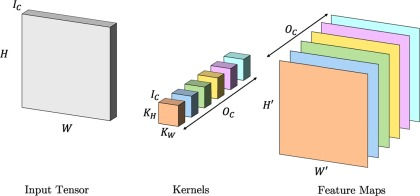
\includegraphics[width=8cm]{assets/images/conv.jpg}
\par\end{centering}
\caption{Example of the convolution operation \cite{Santosh2022-2}}
\label{fig:convolution}
\end{figure}

The field of view of a single kernel is small, as typically kernels of size $3\times3$, $5\times5$, or $7\times7$ are used \cite{Santosh2022-2}. In order to address this issue and to be able to build up and capture more complex features in the subsequent layers, the pooling layer is often added. The pooling layer effectively downsamples the feature maps, commonly by a factor of two. This allows the next convolution layers to learn more abstract features that were further apart in the previous feature map. In order to compensate to the information lost during the downsampling, usually a number of independent kernels is increased for the next convolutions after each pooling layer. During pooling, a small array slides over the input map and always selects only a single value from the area it covers, hence decreasing the size of the map. Two pooling methods are common:

\begin{enumerate}
    \item Max pooling selects the maximal value from the area it covers, and
    \item Average pooling computes the mean from the values it covers.
\end{enumerate}

Example of pooling operations, both max and average, can be seen in the figure \ref{fig:pooling}.

\begin{figure}[H]
\begin{centering}
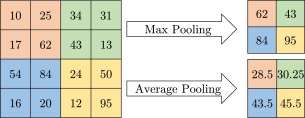
\includegraphics[width=8cm]{assets/images/pooling.jpg}
\par\end{centering}
\caption{Example of max and average pooling operations \cite{Santosh2022-2}}
\label{fig:pooling}
\end{figure}
% importance for image analysis, concept (cat), how they work, how they can be used in medicine, limitations

\subsection{U-Net}
% architecture, advantages, limitations

\subsection{Vision Transformer}
% architecture, advantages, limitations

\section{Challenges, Strategies and Future}

\subsection{Data Annotation}
% how data is annotated, problems limitations etc

\subsection{Weakly Supervised Learning}
% what it is, how it works, challenges

\subsection{Active Learning}
% what it is, how ut works, why it is important, explainability

\subsection{Future Trends}
% what to expect next

